\clearpage
\section{Aufbau und Durchführung}
\subsection{Aufbau}
Der Aufbau ist in Abb. \ref{fig:aufbau} schematisch dargestellt. Die SQUID-Sonde wird in einem Behälter durch flüssigen Stickstoff unter die kritische Temperatur gebracht und über die Auswerteelektronik mit dem Oszilloskop verbunden, welches per Computer ausgelesen wird. Die jeweiligen Probe wird an einem motorgesteuerten Dreharm angebracht und unterhalb der Sonde platziert. Zur Messung stehen fünf Widerstände, welche in einem Stromkreis mit der Leiterschleife in Reihe geschaltet werden, sowie weiter Proben mit unbekannten Dipolmomenten zur Verfügung.\\
\begin{figure}[h]
\begin{center}
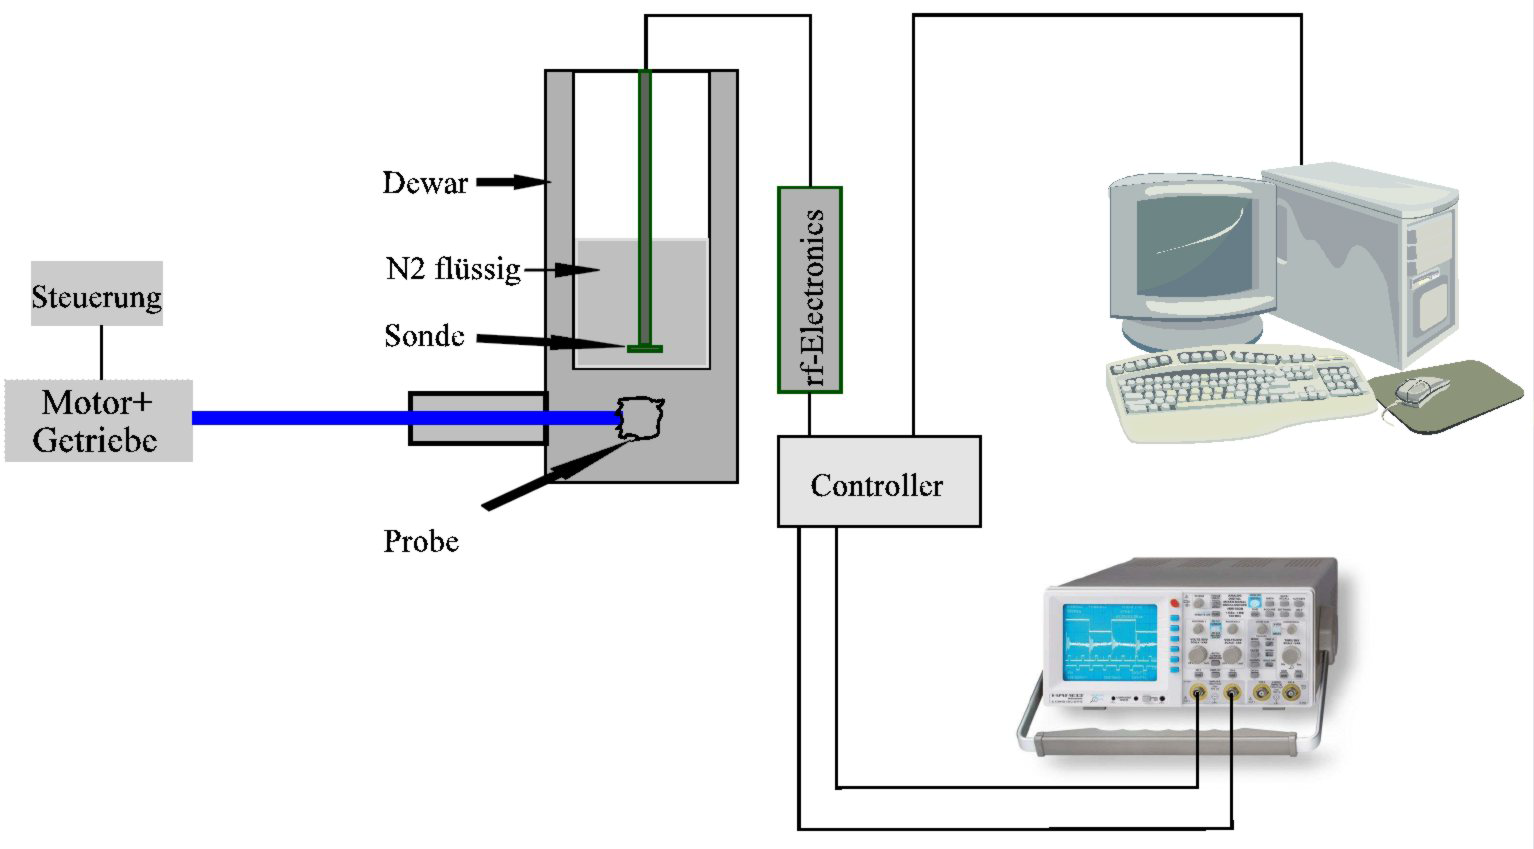
\includegraphics[scale=0.3]{aufbau}
\caption{Schematischer Versuchsaufbau. Quelle: [ver]}
\label{fig:aufbau}
\end{center}
\end{figure}
Am PC können über das JSQ-Magnetometer verschiedene Parameter des Schwingkreises am SQUID variiert werden. VCA bezeichnet die Amplitude, VCO die Frequenz des Schwingkreises. Über OFF kann der Offset der Amplitude eingestellt werden, mit Integr.C wird die Signalglättung bestimmt. FB-R (Feedback-Resistor) bestimmt den Widerstand der Schaltung und somit den Verstärkungsgrad.
\subsection{Durchführung}
Vor Beginn der Messung muss der Stickstoff in den Kryostat eingefüllt werden, damit der Supraleiter unter seine kritische Temperatur gekühlt wird. Für spätere Berechnungen muss der Abstand zwischen SQUID-Sonde und Probe bestimmt werden, sowie der Radius der Leiterschleife und die an der Leiterschleife anliegende Spannung.\\
Bevor nun Messungen durchgeführt werden können, muss der Arbeitspunkt gewählt werden. Dazu muss die Amplitude des SQUID-Patterns über die Einstellungen des JSQ maximiert werden. Dieses entsteht, wenn im Schwingkreis zusätzlich zur oszillierenden eine Dreiecksspannung eingekoppelt wird. Dabei entsteht im SQUID eine Flussänderung über mehrere $\Phi_0$, die dabei gemessene Spannung wird SQUID-Pattern genannt.\\
\begin{figure}[h]
\begin{center}
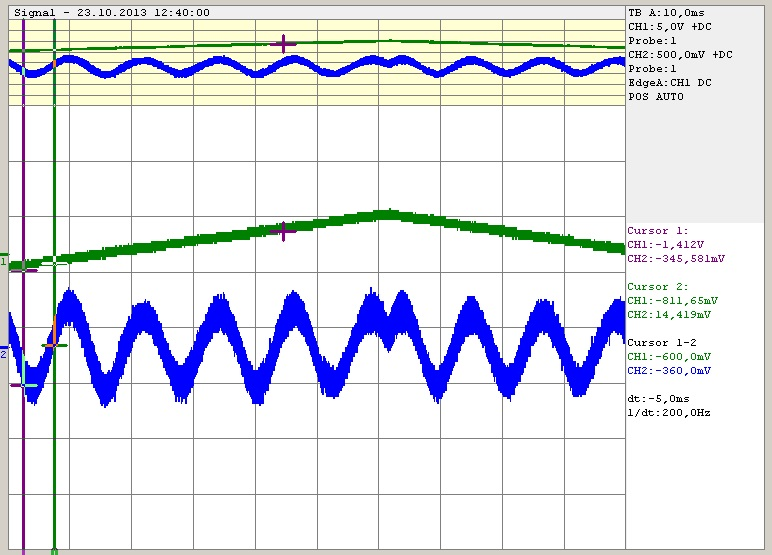
\includegraphics[scale=0.5]{justierung}
\caption{SQUID-Pattern nach der Justierung}
\label{fig:pattern}
\end{center}
\end{figure}
Ist das Pattern gut zu sehen, kann die eigentliche Messung beginnen. In Abb. \ref{fig:pattern} kann man unser SQUID-Pattern nach der Justierung sehen. Dafür wird die Leiterschleife mit verschieden Widerständen in den Versuchsaufbau gebracht und über den Motor rotiert. Um später daraus die Dipolmomente/Feldstärken zu berechnen werden die am Oszilloskop aufgeszeichneten Spannungsverläufe am PC ausgelesen und gespeichert. Das selbe wird mit einigen Proben unbekannter Feldstärken wiederholt, in unserem Fall konnte dies nur mit einer Probe, dem Magnetospan, durchgeführt werden da die Versuchsanordnung einen Fehler auf wies welcher nicht vor Ort und der gegebenen Zeit repariert werden konnte, weshalb der Versuch abgebrochen werden musste. Zusätzlich werden die aufgenommenen Verläufe noch in Polardiagrammen dargestellt.
